\section{Constraints}

From the previous sections one might obtain the impression that all problems in mechanics have been reduced to solving the set of differential equations~\eqref{eq:1.19}:
\begin{equation*}
    m_i\ddot{\symbf{r}}_i=\symbf{F}_i^{\left(e\right)}+\sum_j\symbf{F}_{ji}.
\end{equation*}
One merely substitutes the various forces acting upon the particles of the system, turns the mathematical crank, and grinds out the answers! Even from a purely physical standpoint, however, this view is oversimplified. For example, it may be necessary to take into account the \emph{constraints} that limit the motion of the system. We have already met one type of system involving constraints, namely rigid bodies, where the constraints on the motions of the particles keep the distances \(r_{ij}\) unchanged. Other examples of constrained systems can easily be furnished. The beads of an abacus are constrained to one-dimensional motion by the supporting wires. Gas molecules within a container are constrained by the walls of the vessel to move only \emph{inside} the container. A particle placed on the surface of a solid sphere is subject to the constraint that it can move only on the surface or in the region exterior to the sphere.

Constraints may be classified in various ways, and we shall use the following system. If the conditions of constraint can be expressed as equations connecting the coordinates of the particles (and possibly the time) having the form
\begin{equation}
    f\left(\symbf{r}_1,\symbf{r}_2,\symbf{r}_3,\ldots,t\right)=0,\label{eq:1.37}
\end{equation}
then the constraints are said to be \emph{holonomic}. Perhaps the simplest example of holonomic constraints is the rigid body, where the constraints are expressed by equations of the form
\begin{equation*}
    \left(\symbf{r}_i-\symbf{r}_j\right)^2-c_{ij}^2=0.
\end{equation*}
A particle constrained to move along any curve or on a given surface is another obvious example of a holonomic constraint, with the equations defining the curve or surface acting as the equations of a constraint.

Constraints not expressible in this fashion are called nonholonomic. The walls of a gas container constitute a nonholonomic constraint. The constraint involved in the example of a particle placed on the surface of a sphere is also nonholonomic, for it can be expressed as an inequality
\begin{equation*}
    r^2-a^2\geqslant0
\end{equation*}
(where \(a\) is the radius of the sphere), which is not in the form of \eqref{eq:1.37}. Thus, in a gravitational field a particle placed on the top of the sphere will slide down the surface part of the way but will eventually fall off.

Constraints are further classified according to whether the equations of constraint contain the time as an explicit variable (rheonomous) or are not explicitly dependent on time (scleronomous). A bead sliding on a rigid curved wire fixed in space is obviously subject to a scleronomous constraint; if the wire is moving in some prescribed fashion, the constraint is rheonomous. Note that if the wire moves, say, as a reaction to the bead's motion, then the time dependence of the constraint enters in the equation of the constraint only through the coordinates of the curved wire (which are now part of the system coordinates). The overall constraint is then scleronomous.

Constraints introduce two types of difficulties in the solution of mechanical problems. First, the coordinates \(r_i\) are no longer all independent, since they are connected by the equations of constraint; hence the equations of motion \eqref{eq:1.19} are not all independent. Second, the forces of constraint, e.g., the force that the wire exerts on the bead (or the wall on the gas particle), is not furnished a priori. They are among the unknowns of the problem and must be obtained from the solution we seek. Indeed, imposing constraints on the system is simply another method of stating that there are forces present in the problem that cannot be specified directly but are known rather in terms of their effect on the motion of the system.

In the case of holonomic constraints, the first difficulty is solved by the introduction of \emph{generalized coordinates}. So far we have been thinking implicitly in terms of Cartesian coordinates. A system of \(N\) particles, free from constraints, has \(3N\) independent coordinates or \emph{degrees of freedom}. If there exist holonomic constraints, expressed in \(k\) equations in the form \eqref{eq:1.37}, then we may use these equations to eliminate \(k\) of the \(3N\) coordinates, and we are left with \(3N-k\) independent coordinates, and the system is said to have \(3N-k\) degrees of freedom. This elimination of the dependent coordinates can be expressed in another way, by the introduction of new, \(3N-k\), independent variables \(q_1\), \(q_2\), \(\ldots\), \(q_{3N-k}\) in terms of which the old coordinates \(\symbf{r}_1\), \(\symbf{r}_2\), \(\ldots\), \(\symbf{r}_N\) are expressed by equations of the form
\begin{equation}
    \begin{aligned}
        \symbf{r}_1&=\symbf{r}_1\left(q_1,q_2,\ldots,q_{3N-k},t\right),\\
        &\vdotswithin{=}\\
        \symbf{r}_N&=\symbf{r}_N\left(q_1,q_2,\ldots,q_{3N-k},t\right)
    \end{aligned}
    \label{eq:1.38}
\end{equation}
containing the constraints in them implicitly. These are \emph{transformation} equations from the set of \(\left(\symbf{r}_l\right)\) variables to the \(\left(q_l\right)\) set, or alternatively Eqs.~\eqref{eq:1.38} can be considered as parametric representations of the \(\left(\symbf{r}_l\right)\) variables. It is always assumed that we can also transform back from the \(\left(q_l\right)\) to the \(\left(\symbf{r}_l\right)\) set, i.e., that Eqs.~\eqref{eq:1.38} combined with the \(k\) equations of constraint can be inverted to obtain any \(q_i\) as a function of the \(\left(\symbf{r}_l\right)\) variable and time.

Usually the generalized coordinates, \(q_l\), unlike the Cartesian coordinates, will not divide into convenient groups of three that can be associated together to form vectors. Thus, in the case of a particle constrained to move \emph{on} the surface of a sphere, the two angles expressing position on the sphere, say latitude and longtude, are obvious possible generalized coordinates. Or, in the example of a double pendulum moving in a plane (two particles connected by an inextensible light rod and suspended by a similar rod fastened to one of the particles), satisfactory generalized coordinates are the two angles \(\theta_1\), \(\theta_2\). (Cf. Fig.~\ref{fig:1.4}.) Generalized coordinates, in the sense of coordinates other than Cartesian, are often useful in systems without constraints. Thus, in the problem of a particle moving in an external central force field (\(V=V\left(r\right)\)), there is no constraint involved, but it is clearly more convenient to use spherical polar coordinates than Cartesian coordinates. Do not, however, think of generalized coordinates in terms of conventional orthogonal position coordinates. All sorts of quantities may be invoked to serve as generalized coordinates. Thus, the amplitudes in a Fourier expansion of \(\symbf{r}_j\) may be used as generalized coordinates, or we may find it convenient to employ quantities with the dimensions of energy or angular momentum.

\begin{figure}[htbp]
    \centering
    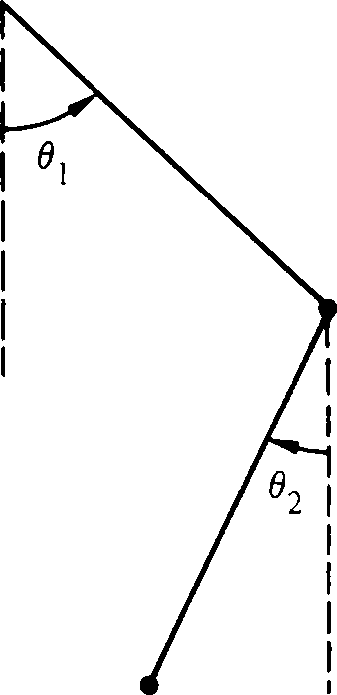
\includegraphics[scale = 0.225]{01/figures/1.4}
    \caption{Double pendulum.}
    \label{fig:1.4}
\end{figure}

If the constraint is nonholonomic, the equations expressing the constraint cannot be used to eliminate the dependent coordinates. An oft-quoted example of a nonholonomic constraint is that of an object rolling on a rough surface without slipping. The coordinates used to describe the system will generally involve angular coordinates to specify the orientation of the body, plus a set of coordinates describing the location of the point of contact on the surface. The constraint of ``rolling" connects these two sets of coordinates; they are not independent. A change in the position of the point of contact inevitably means a change in its orientation. Yet we cannot reduce the number of coordinates, for the ``rolling" condition is not expressible as a equation between the coordinates, in the manner of \eqref{eq:1.37}. Rather, it is a condition on the \emph{velocities} (i.e., the point of contact is stationary), a differential condition that can be given in an integrated form only \emph{after} the problem is solved.

A simple case will illustrate the point. Consider a disk rolling on the horizontal \(xy\) plane constrained to move so that the plane of the disk is always vertical. The coordinates used to describe the motion might be the \(x\), \(y\) coordinates of the center of the disk, an angle of rotation \(\phi\) about the axis of the disk, and an angle \(\theta\) between the axis of the disk and say, the \(x\) axis (cf. Fig~\ref{fig:1.5}). As a result of the constraint the velocity of the center of the disk, \(\symbf{v}\), has a magnitude proportional to \(\dot{\phi}\),
\begin{equation*}
    v=a\dot{\phi},
\end{equation*}
where \(a\) is the radius of the disk, and its direction is perpendicular to the axis of the disk:
\begin{equation*}
    \begin{aligned}
        \dot{x}&=v\sin\theta,\\
        \dot{y}&=-v\cos\theta.
    \end{aligned}
\end{equation*}
Combining these conditions, we have two \emph{differential} equations of constraint:
\begin{equation}
    \begin{aligned}
        \odif{x}-a\sin\theta\odif{\phi}&=0,\\
        \odif{y}+a\cos\theta\odif{\phi}&=0.
    \end{aligned}
    \label{eq:1.39}
\end{equation}
Neither of Eqs.~\eqref{eq:1.39} can be integrated without in fact solving the problem; i.e., we cannot find an integrating factor \(f\left(x,y,\theta,\phi\right)\) that will turn either of the equations into perfect differentials (cf. Derivation~\ref{derivation:1.4}).\footnote{In principle, an integrating factor can always be found for a first-order differential equation of constraint in systems involving only two coordinates and such constraints are therefore holonomic. A familiar example is the two-dimensional motion of a circle rolling on an inclined plane.} Hence, the constraints cannot be reduced to the form of Eq.~\eqref{eq:1.37} and are therefore nonholonomic. Physically we can see that there can be no direct functional relation between \(\phi\) and the other coordinates \(x\), \(y\), and \(\theta\) by noting that at any point on its path the disk can be made to roll around in a circle tangent to the path and of arbitrary radius. At the end of the process, \(x\), \(y\), and \(\theta\) have been returned to their original values, but \(\phi\) has changed by an amount depending on the radius of the circle.

\begin{figure}[htbp]
    \centering
    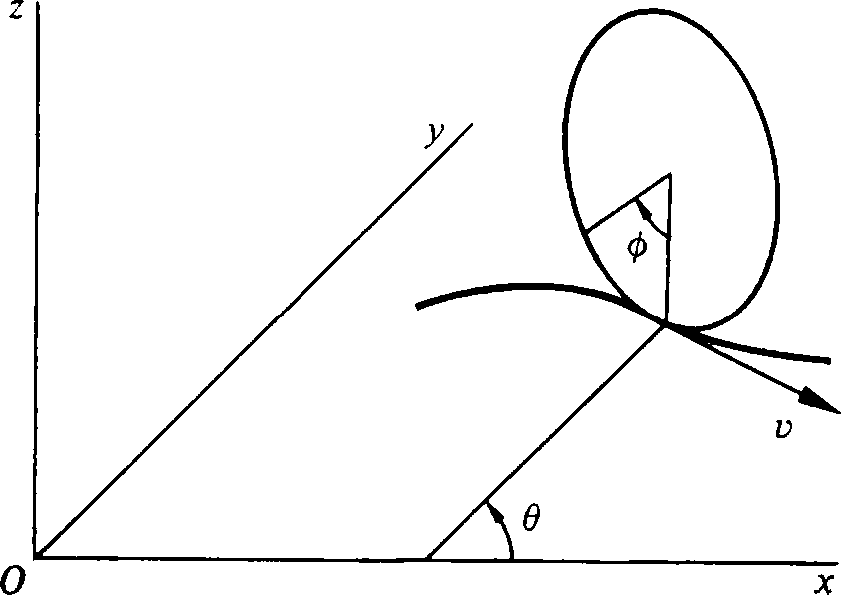
\includegraphics[scale = 0.225]{01/figures/1.5}
    \caption{Vertical disk rolling on a horizontal plane.}
    \label{fig:1.5}
\end{figure}

Nonintegrable \emph{differential} constraints of the form of Eqs.~\eqref{eq:1.39} are of course not the only type of nonholonomic constraints. The constraint conditions may involve higher-order derivatives, or may appear in the form of inequalities, as we have seen.

Partly because the dependent coordinates can be eliminated, problems involying holonomic constraints are always amenable to a formal solution. But there is no general way to attack nonholonomic examples. True, if the constraint is nonintegrable, the differential equations of constraint can be introduced into the problem along with the differential equations of motion, and the dependent equations eliminated, in effect, by the method of Lagrange multipliers.

We shall return to this method at a later point. However, the more vicious cases of nonholonomic constraint must be tackled individually, and consequently in the development of the more formal aspects of classical mechanics, it is almost invariably assumed that any constraint, if present, is holonomic. This restriction does not greatly limit the applicability of the theory, despite the fact that many of the constraints encountered in everyday life are nonholonomic. The reason is that the entire concept of constraints imposed in the system through the medium of wires or surfaces or walls is particularly appropriate only in macroscopic or large-scale problems. But today physicists are more interested in atomic and nuclear problems. On this scale all objects, both in and out of the system, consist alike of molecules, atoms, or smaller particles, exerting definite forces, and the notion of constraint becomes artificial and rarely appears. Constraints are then used only as mathematical idealizations to the actual physical case or as classical approximations to a quantum-mechanical property, e.g., rigid body rotations for ``spin." Such constraints are always holonomic and fit smoothly into the framework of the theory.

To surmount the second difficulty, namely, that the forces of constraint are unknown a priori, we should like to so formulate the mechanics that the forces of constraint disappear. We need then deal only with the known applied forces. A hint as to the procedure to be followed is provided by the fact that in a particular system with constraints, i.e., a rigid body, the work done by internal forces (which are here the forces of constraint) vanishes. We shall follow up this clue in the ensuing sections and generalize the ideas contained in it.
